\let\negmedspace\undefined
\let\negthickspace\undefined
\documentclass[journal]{IEEEtran}
\usepackage[a5paper, margin=10mm, onecolumn]{geometry}
%\usepackage{lmodern} % Ensure lmodern is loaded for pdflatex
\usepackage{tfrupee} % Include tfrupee package

\setlength{\headheight}{1cm} % Set the height of the header box
\setlength{\headsep}{0mm}     % Set the distance between the header box and the top of the text

\usepackage{gvv-book}
\usepackage{gvv}
\usepackage{cite}
\usepackage{amsmath,amssymb,amsfonts,amsthm}
\usepackage{algorithmic}
\usepackage{graphicx}
\usepackage{textcomp}
\usepackage{xcolor}
\usepackage{txfonts}
\usepackage{listings}
\usepackage{enumitem}
\usepackage{mathtools}
\usepackage{gensymb}
\usepackage{comment}
\usepackage[breaklinks=true]{hyperref}
\usepackage{tkz-euclide} 
\usepackage{listings}
% \usepackage{gvv}                                        
\def\inputGnumericTable{}                                 
\usepackage[latin1]{inputenc}                                
\usepackage{color}                                            
\usepackage{array}                                            
\usepackage{longtable}                                       
\usepackage{calc}                                             
\usepackage{multirow}                                         
\usepackage{hhline}                                           
\usepackage{ifthen}                                           
\usepackage{lscape}
\begin{document}

\bibliographystyle{IEEEtran}
\vspace{3cm}

\title{12.9.2.2}
\author{EE24BTECH11013 - MANIKANTA D}
% \maketitle
% \newpage
% \bigskip
{\let\newpage\relax\maketitle}

\renewcommand{\thefigure}{\theenumi}
\renewcommand{\thetable}{\theenumi}
\setlength{\intextsep}{10pt} % Space between text and floats


\numberwithin{equation}{enumi}
\numberwithin{figure}{enumi}
\renewcommand{\thetable}{\theenumi}

\textbf{Question:}\\
Consider the differential equation 
\begin{align}
    y^\prime - 2x - 2 = 0
\end{align}
Verify that
\begin{align}
    y = x^2 + 2x + C
\end{align}
is a solution for it.\\
\textbf{Theoretical Solution:}

The given differential equation is:
\begin{align}
    y^\prime - 2x - 2 = 0
\end{align}

Rearrange the terms to group all  $x$ and $y$related terms:
\begin{align}
    y^\prime = 2x + 2
\end{align}

Now integrate both sides with respect to $x$:
\begin{align}
    \int y^\prime dx = \int \brak{2x + 2} dx
\end{align}

The left-hand side simplifies to  $y$, and the right-hand side is integrated term by term:
\begin{align}
    y = \int 2x dx + \int 2 dx \\
    y = x^2 + 2x + C
\end{align}

This matches the assumed solution:
\begin{align}
    y = x^2 + 2x + C
\end{align}
\textbf{Integrating Factor Approach:}
\begin{align}
    y^\prime - 2x = 2
\end{align}

Rearrange to match the standard form:
\begin{align}
    y^\prime = 2x + 2
\end{align}

Integrate both sides:
\begin{align}
    y = \int (2x + 2) dx \\
    y = x^2 + 2x + C
\end{align}

Thus, we recover the same solution:
\begin{align}
    y = x^2 + 2x + C
\end{align}
 \textbf{ Difference equation method }\\
The difference equation is:
\begin{align}
y_{n+1} = y_n + h \cdot y'(x),
\end{align}
where:
\begin{itemize}
    \item  $y_n$ is the value of the function at step  $n$,
    \item $h$ is the step size,
    \item $y'\brak{x}$ is the derivative of the function.
\end{itemize}
\subsection*{Step 1: Substitute $y_n$ and $y'(x)$}
Assume $y_n = x_n^2 + 2x_n + C$. Substituting  $y'\brak{x} = 2x_n + 2$ into the difference equation gives:
\begin{align}
y_{n+1} = y_n + h \cdot (2x_n + 2).
\end{align}
Substituting  $y_n = x_n^2 + 2x_n + C $, we get:
\begin{align}
y_{n+1} = (x_n^2 + 2x_n + C) + h \cdot (2x_n + 2).
\end{align}

\subsection*{Step 2: Expand  $y_{n+1}$}
Expanding the terms:
\begin{align}
y_{n+1} = x_n^2 + 2x_n + C + 2hx_n + 2h,
\end{align}
\begin{align}
y_{n+1} = x_n^2 + (2x_n + 2hx_n) + (C + 2h).
\end{align}
\subsection*{Step 3: Difference Equation Solution}
Starting with the expanded difference equation:
\begin{align}
y_{n+1} = x_n^2 + (2x_n + 2hx_n) + (C + 2h).
\end{align}
We can further simplify by grouping terms:
\begin{align}
y_{n+1} = x_n^2 + 2x_n(1 + h) + (C + 2h).
\end{align}

Thus, the solution for $ y_{n+1} $ becomes:
\begin{align}
y_{n+1} = x_n^2 + 2x_n(1 + h) + (C + 2h).
\end{align}
This matches the original function $y = x^2 + 2x + C$ when $h \to 0.15$, verifying the consistency of the difference equation method with the exact solution.
\begin{figure}[h]
    \centering
    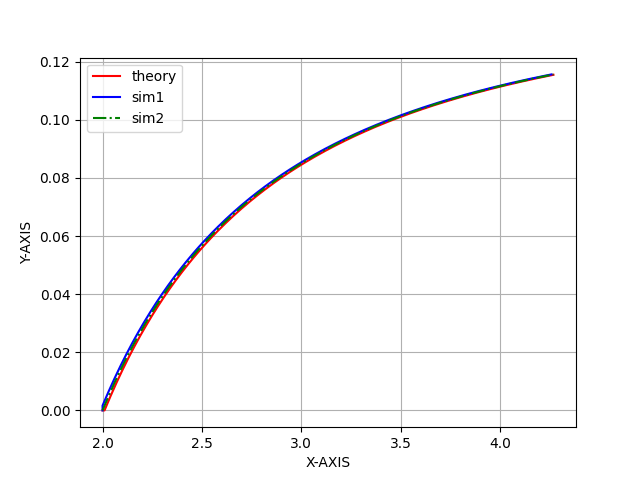
\includegraphics[width=\columnwidth]{fig.png}
    \caption{Plot of the differential equation}
    \label{fig:Plot}
    \end{figure}
\end{document}}
